\section{06.11.23 : Twierdzenie Dooba o zatrzymaniu, czyli jak uprawiać hazard}

%\begin{definition}
  Dla $T:\Omega\to\N$ i procesu $\{X_n\}$ definiujemy zmienną $X_T$ wzorem
  $$X_T(\omega)=X_{T(\omega)}(\omega)$$

  Dla martyngału $\{X_n\}_{n\in\N}$ i czasu zatrzymania $T$ rozważamy ciąg zmiennych $\{X_{n\land T}\}_{n\in\N}$
  $$\color{blue}X_{n\land T}(\omega)=\begin{cases}X_n& n\leq T(\omega)\\ X_{T(\omega)}(\omega) & n\geq T(\omega) \end{cases}$$
%\end{definition}

  Tutaj dla $X,y\in\R$ piszemy $x\land y$ aby przekazać, że interesuje nas $\min\{x,y\}$. To znaczy $x\land y=\min\{x,y\}$.

Czyli gramy w pewna uczciwą grę i mamy strategię wyjścia $T$, ale musimy np. zdążyć na obiad, więc chcemy wyjść po co najwyżej $n$ rundach.

\begin{theorem}[Dooba o zatrzymaniu (uproszczone)]
  Niech $\{X_n\}$ będą odpowiednio martyngałem i czasu zatrzymania względem tej samej filtracji $\mathds{F}=\{\set{F}_n\}$. Wówczas proces (ciąg) $\{X_{n\land T}\}$ zdefiniowany wyżej jest martyngałem. W szczególności
  $$\expected{X_{n\land T}}=\expected{X_0}$$
  dla każdego $n$ (średnia jest stała w czasie).
\end{theorem}

\begin{proof}
  Mamy 
  $$X_{n\land T}=\sum_{k=1}^{n\land T}(X_k-X_{k-1})+X_0=\sum_{k=1}^n\mathds{1}_{T\geq k}(X_k-X_{k-1})+X_9$$
  gdzie
  $$\mathds{1}_{T\geq k}=1-\mathds{1}_{T<k}=1-1_{T\leq k-1}\in \set{F}_{k-1}$$
  i teza wynika z przykładu o transformacie martyngałowej.
\end{proof}

\begin{example}
  \item Gracz rozpoczyna grę z kapitałem $j\$$. W każdym rozdaniu może z prawdopodobieństwem $\frac{1}{2}$ zyskać jednego dolara lub go stracić. Celem gracza jest wzbogacenie się o $k$ dolarów. Jakie jest prawdopodobieństwo sukcesu $p_{k,j}$?

    Zaczynamy w punkcie $j$ i chcemy dojść do punktu $j+k$, a boimy się punktu $0$

    \begin{center}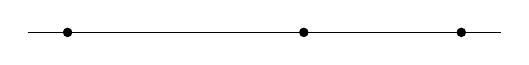
\begin{tikzpicture}
      \draw (-0.5, 0)--(5.5, 0);
      \filldraw (0, 0) circle (1.5pt);
      \filldraw (5, 0) circle (1.5pt);
    \filldraw(3, 0) circle (1.5pt);
    \end{tikzpicture}\end{center}

    Niech $\{\xi_k\}$ będą niezależne o tym samym rozkładzie $\prob{\xi_k=\pm 1}=\frac{1}{2}$. Rozważmy
    $$X_n=\sum_{k=1}^n\xi_n.$$
    Żeby rozwiązać to zadanie to chcemy rozważyć funkcję
    $$T=\inf\{n\in\N\;:\; X_n=-j\text{ lub }X_n=k\}$$
    Teraz szukane przez nas prawdopodobieństwo to
    $$p_{k,j}=\prob{X_T=k}$$

    Rozważamy filtrację $\mathds{F}=\{\set{F}_n\},\; \set{F}_n=\sigma(\xi_1,...,\xi_n)$. Ciąg $\{X_n\}$ jest $\mathds{F}$-adaptowalny, więc $T$ jest $\mathds{F}$-czasem zatrzymania.

    Ciąg $\{X_n\}$ jest $\mathds{F}$-martyngałem, co wynika z faktu, że $\xi_{n+1}$ są niezależne od $\set{F}_n$ i mają $\expected$ równą $0$:
    $$\expected{X_{n+1}}{\set{F}_n}=\expected{\xi_{n+1}+X_n}{\set{F}_n}=\expected{\xi_{n+1}}+\expected{X_n}{\set{F}_n}=0+X_n$$
    Z twierdzenia o zatrzymaniu wiemy więc, że
    $$\expected{X_{n\land T}}=\expected{X_0}=0$$
    i tutaj szkopuł jest taki, że nas interesuje $X_T$ a nie $X_{n\land T}$. Musimy więc przejść z $n$ do nieskończoności.

    W pierwszej kolejności chcemy się upewnić, że $\prob{T<\infty}=1$, bo 
    $$\prob{T\geq n}\leq \prob{|X_n|\leq k+j}=\prob{\frac{|X_n|}{\sqrt{n}}\leq \frac{j+k}{\sqrt{n}}}\xrightarrow{CTG} 0$$
    a ponieważ
    $$\prob{T=\infty}=\lim_{n\to\infty}\prob{T\geq n}=0.$$
    W takim razie ciąg $X_{n\land T}$ zbiega prawie wszędzie do ciągu $X_T$. Mało tego, dla pewnego $n$ się zacznie stabilizować. Pozostaje uzasadnić, że możemy wejść z granicą pod całkę, ale to wynika z faktu, że
    $$|X_{n\land T}|\leq j+k,$$
    więc mamy
    $$0=\expected{X_0}=\lim \expected{X_{n\land T}}=\expected{\lim X_{n\land T}}=\expected{X_T}.$$
    Rozpisując już na końcu
    \begin{align*}
      0=\expected{X_T}&=k\prob{X_T=k}-j\prob{X_T=-j}=k\cdot p_{k,j}-j(1-p_{k,j})
    \end{align*}
    co pozwala nam wyliczyć
    $$p_{k,j}=\frac{j}{k+j}.$$

    W szczególności mamy
    \begin{align*}
      \prob{\{X_n\}\text{ osiągnie k}}&=\lim_{j\to\infty}\prob{\{X_k\}\text{ osiągnie k przed osiągnięciem -j}}=\\ 
                                      &=\lim_{j\to\infty}p_{k,j}=\lim_{j\to\infty}\frac{j}{j+k}=1
    \end{align*}
  \item Gracz rozpoczyna grę z kapitałem $j\$$. W każdym rozdaniu może z prawdopodobieństwem $p$ zyskać jednego dolara lub stracić go z prawdopodobieństwem $(1-p)$. Celem gracza jest wzbogacenie się o $k$ dolarów. Jakie jest prawdopodobieństwo sukcesu $p_{k,j}$ gdy $p>\frac{1}{2}$?

    Jest to niemalże takie samo zadanie jak wcześniej, z tym że tym razem nie mamy martyngału. Niemniej jednak modelować będziemy to w niemalże identyczny sposób.

    Niech $\{\eta_k\}$ będą iid takie, że $\prob{\eta_k=1}=p$ oraz $\prob{\eta_k=-1}=1-p$. Określamy $X_n=\sum_{k=1}^n\eta_k$. Mamy wówczas
    \begin{align*}
      \expected{X_{n+1}}{\set{F}_n}&=\expected{\eta_{n+1}}+X_n=X_n+(2p-1)>X_n
    \end{align*}
    czy $\{X_n\}$ jest podmartyngałem. Określmy czas zatrzymania
    $$T=\inf\{n\;:\;X_n=-j\text{ lub }X_n=k\}.$$

    Chcemy sobie zorganizować nowy martyngał postaci
    $$M_n=f(X_n)$$
    dla pewnej funkcji $f:\Z\to\R$ takiej, że
    $$\expected{M_{n+1}}{\set{F}_n}=M_n.$$
    Mamy
    \begin{align*}
      \expected{M_{n+1}}{\set{F}_n}&=\expected{f(X_n+\eta_{n+1}}{\set{F}_n}=\\ 
                                   &=F(X_n),
    \end{align*}
    gdzie $F(x)=\expected{f(x+\eta_{n+1})}=pf(x+1)+(1-p)f(x-1)$ jest oznaczeniem pomocniczym przy "odcałkowaniu niezależnej $\eta_{n+1}$".

    Aby $\{M_n\}$ był martyngałem musi zachodzić
    $$M_n=f(X_n)=pf(X_n+1)+(1-p)f(X_n-1)=F(X_n)=\expected{M_{n+1}}{\set{F}_n}$$
    $f$ musi zatem spełniać rekurencję
    $$f(x)=pf(x+1)+(1-p)f(x-1)$$
    Szukamy rozwiązania postaci $f(x)=\gamma^x$. Mamy więc
    $$\gamma^x=p\gamma^{x+1}+(1-p)\gamma^{x-1}$$
    $$\gamma=p\gamma^2+(1-p)$$
    i istnieją dwa rozwiązania: $\gamma=1$ oraz $\gamma=\frac{1-p}{p}$. Wówczas
    $$M_n=f(X_n)=\left(\frac{1-p}{p}\right)^{X_n}$$
    jest martyngalem. Znowu $M_{n\land T}\leq\left(\frac{p}{1-p}\right)^{k+j}$, a z twierdzenia Dooba
    $$\expected{M_{n\land T}}=\expected{M_0}=1$$
    i poprzez przejście graniczne
    $$\expected{M_T}=1$$
    Oznaczamy $\prob{X_T=k}=r_{j,j}$ i mamy
    $$1=\expected{M_T}=\gamma^{-j}(1-r_{k,j})+\gamma^kr_{k,j}$$
    gdzie
    $$r_{k,j}=\frac{1-\gamma^{-j}}{\gamma^k-\gamma^{j-1}}$$
    w szczególności
    $$\prob{\{X_n\}\text{ osiągnie k}}=\lim_{j\to\infty} r_{j,k}=1$$
    $$\prob{\{X_n\}\text{ osiągnie j}}=\lim_{k\to\infty}(1-r_{k,j})=\lim_{k\to\infty}...=\gamma^j$$

  \item Rozważmy $X_n=\sum Y_k$, gdzie $Y_k$ są iid takie, że $\prob{Y_1=\pm 1}=\frac{1}{2}$. To znaczy, że jeden gracz bierze udział w uczciwej grze i obstawiamy.
\end{example}
